% group articles by domain 
% for every article write a short summary of its relevant features
% and add an illustrative picture
% then criticize the presented solutions

\subsection{Representing Urban Scenery}
In order to obtain an immersive experience, there's a number of hardware
setups commonly available:

\begin{floatingfigure}[r]{3cm}
%[r]{5mm}
		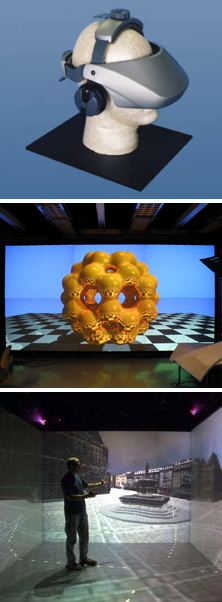
\includegraphics{gfx/hmd-cluster-cave.png}
		\caption{HMD, Cluster, CAVE}
		\label{FIG-HMD-CLUSTER-CAVE}
	\end{floatingfigure}

\begin{description}
	\item[Head Mounted Display (HMD)] --
	  Head mounting displays are shaped like glasses.
	  They normally feature a gyroscope or similar device to measure head orientation and tilt.
	  
		Using a head mounted display has the benefit of sticking to the user's head
		and detecting head orientation.
		On the other hand each HMD serves one single user.
		Additionally most users report suffering from fatigue after long periods of
		usage and it has limited resolution.
			
	\item[Cave Automatic Virtual Environment (CAVE)] --
	  A CAVE is an immersive virtual reality environment where projectors are directed to four,
	  five or six of the walls of a room-sized cube.
	  
		Shares with HMDs the benefit of enclosing the user's viewing area.
		Has a better resolution though. The downside is the small number of simultaneous users who
		can experience the CAVE at the same time.
	
	\item[Wall] --
	  TODO
	  
		Its size and resolution depend entirely on the setup, but normally a wall offers high resolution
		(depends on the number of projectors in the grid and their resolution).
		The presence of a wall doesn't limit the number of users.
		The downside is that users have to face the wall!
\end{description}

Any of these setups is suitable for single user interaction.
In case of a reviewing session, in which at least two participants are required,
CAVE or Wall are better suited.

Using a Wall or CAVE presents other challenges: the computers responsible for
generating each projectors' images must be synchronized, its' color parameters calibrated,
the viewport must be well cropped, etc.
Several systems exist capable of delivering high performance 3D graphics and offering the features mentioned above.
Based on scene graphs there are OpenSceneGraph and OpenSG and others.

The last problem in this category is how to effectively render city landscape.
One has to limit the detail of objects further away.
Ideally the transition should be smooth but recognizing each building's main shape
even far away is equally relevant.
This can be achieved implementing a solution like the following.

\subsubsection{Continuous LOD}
J�rgen D�llner and Henrik Buchholz \cite{LODCITY05} present a
solution for modeling buildings that feature a continuous level of detail.

The authors propose the following levels of detail for a building (derived from
CityGML\footnote{CityGML is a common information model for the representation of 3D urban objects.
It defines the classes and relations for the most relevant topographic objects in cities
and regional models with respect to their geometrical, topological, semantical and appearance properties.
More info at: http://www.citygml.org}, see Figure \ref{FIG-LODCITY}):

\begin{itemize}
	\item simple block model
	\item model with defined roof geometry
	\item detailed indoor and outdoor building features
\end{itemize}

\begin{figure}[htb]
	\centering
	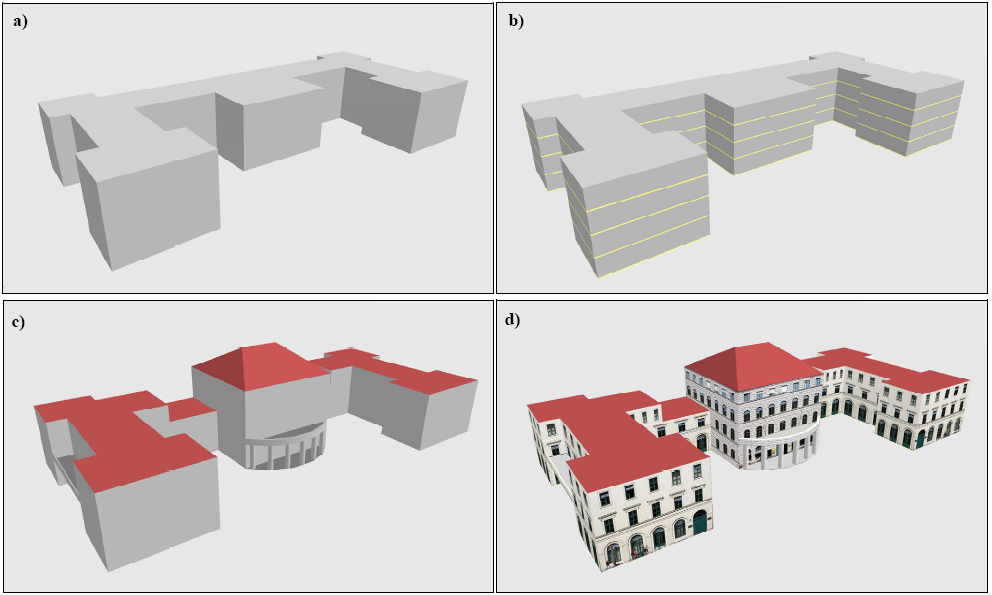
\includegraphics[width=15cm]{gfx/lodcity05-1.png}
	\caption{Continuous LOD: a) block model; b) building split into floors; c) geometry refinement; d) appearance refinement.}
	\label{FIG-LODCITY}
\end{figure}

A building is composed of a list of floor objects. A floor object refers to a floor prototype, which
contains the floor specification. This indirection allows a user to reuse floor prototypes in several
floors of the same building and allows rendering optimizations.

Each floor prototype is defined by its ground plan, which is one or more polygons that define the area
on which walls can be constructed. There can be inner loops in order to allow features like courtyards.
A ground plan supports thickness, useful for defining terraces.

On top of a ground plan one can place walls. A wall represents a vertical, planar polygon.
The default type of wall has no thickness, sufficient if a group of them form a closed surface
and can be only seen from the outside. Thick walls can also be added.
A wall can be lower or higher than its floor height, allowing balcony fronts and chimneys to be defined.

The higher ground plans can have roofs. The most common roof types are supported (hipped, gabled, tent,
mansard, pent, barrel) and a roof is described only by choosing the floor type and placing its
most relevant points (known as the roof skeleton).

Each floor prototype has a related floor decoration. A floor decoration is a collection of facade sections
and window sections. The former allows whole wall sections to be assigned a material while the latter
allows the definition of positioning and appearance of the floor's windows.

TODO: other relevant articles?

\subsection{Getting User Input}
Obtaining user input can happen in an infinity of interface combinations.
In virtual reality the most common solutions may feature:
\begin{itemize}
	\item image processing using camera(s)
	\item speech recognition
	\item motion tracking
	\item space ball, space pilot, etc.
	\item HMD's rotation data
	\item tracked artifacts for direct manipulation
\end{itemize}

The least intrusive interface would use either motion tracking or image processing and speech recognition.
Speech recognition allows commands to be given to the system. The remaining interface allows knowing positioning
and rotation of users or parts of their bodies. Tracking artifacts may either allow the artifact to serve as a
pointer or as a metaphor for direct manipulation.

\subsection{Sketching for Geometry Creation and Editing}

\subsubsection{Smart Sketchpad}
Wenyin et al. created Smart Sketchpad \cite{SMARTSK01}.
Smart Sketchpad recognizes standard shapes (rectangles, triangles, ellipses, straight lines)
and compound shapes such as arrowheads.

Their article describes the steps necessary for shape recognition:
\begin{enumerate}
	\item input as a chain of points
	\item polygonalize to polyline and refine endpoints
	\item close near endpoints - if closed go to step 6
	\item if line ends near another line end, join them and go to step 3
	\item classify line as one of: straight line, polyline or free form curve. go to step 8
	\item close shape recognition *
	\item estimate the parameter of the closed shape
	\item test if shape can be combined with other shapes in the drawing. If so repeat step 8, else end
\end{enumerate}

The $6^{th}$ step was tested with: rule-based system, support vector machine and neural network.
The most successfully approach was SVN, with 97,5\% success, closely followed by NN.

\subsubsection{Assist}
Alvarado and Davis present a work toward an interface for mechanical designers named Assist \cite{FREEDOM01},
with the purpose of allowing them to sketch naturally and have the computer interpreting
their strokes into shapes like rods, hinges, polygons, etc.

The interpretation is a three stages procedure:

\begin{itemize}
	\item match strokes to a series of templates
	\item rank interpretations with several heuristics about drawing style and mechanical engineering
	\item return the most consistent hypothesis
\end{itemize}

Figure \ref{FIG-FREEDOM01} illustrates the result.

The authors emphasize the difficulty they faced when replacing the original human-made stroke
by its computer interpretation. Users prefer composing the whole drawing prior to computer
interpretation replacement. Having the computer interpreting every stroke makes them feel they're
giving up control of the program. Even so, that was the path chosen by the authors because
every extra stroke without giving feedback to the user increases the chance of misinterpretations.
Another relevant conclusion is that users expect symmetry to be kept regarding the interpreted
shapes, so it would be a good idea to detect and suggest alignment restrictions between shapes.

\begin{figure}[htb]
	\centering
	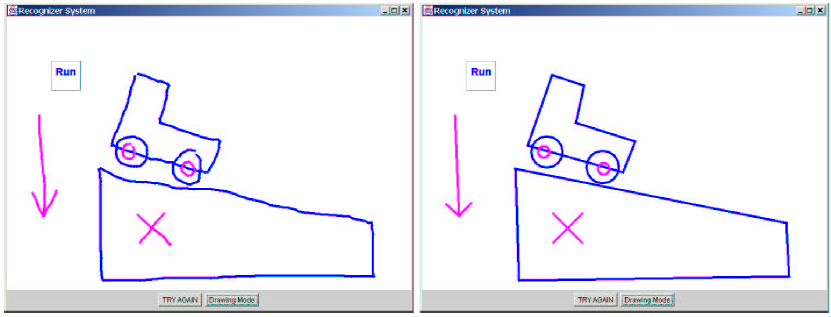
\includegraphics[width=15cm]{gfx/freedom01-1.png}
	\caption{Assist: A car on the hill. Drawn by the user (left), as interpreted and displayed (right).}
	\label{FIG-FREEDOM01}
\end{figure}

\subsubsection{Digital Clay}
Digital Clay \cite{DIGCLAY00} allows a user to draw freely and tries to convert the drawing into a 3D model.
See input and 3D result in Figure \ref{FIG-DIGCLAY}.

It uses two techniques to achieve that:

\begin{itemize}
	\item Huffman-Clowes algorithm, which identifies concave and convex vertices, requiring
	every line to connect to another line and the program additionally demands the object
	drawn to be solid;
	\item infers 3D coordinates based on inherent rules that govern each type of drawing projection.
	Examples: axes of isometric drawings have equal angles between them;
	perspective drawings show foreshortening of lines as we get closer to the viewer.
\end{itemize}

The downfalls of this method are the impossibility of describing occluded faces and the limited
editing capacities available once the conversion has been done.

\begin{figure}[htb]
	\centering
	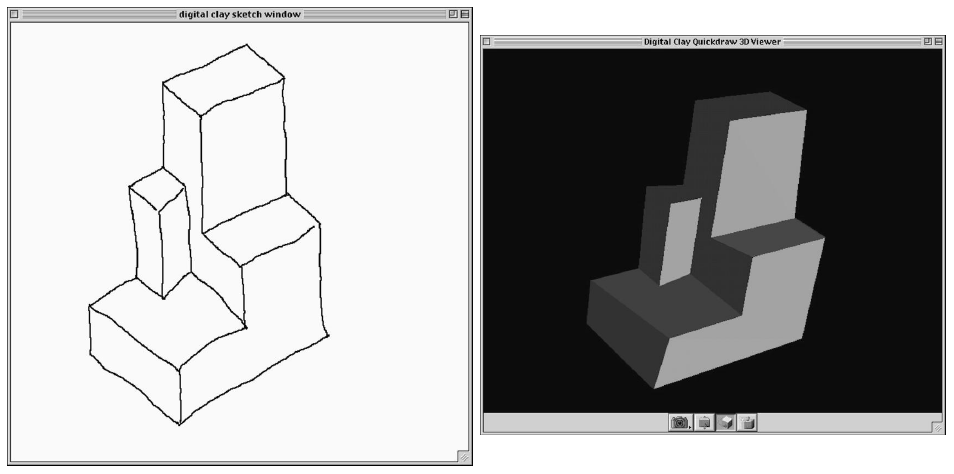
\includegraphics[width=15cm]{gfx/digclay00-1.png}
	\caption{Digital Clay: Raw sketch input and its 3D interpretation.}
	\label{FIG-DIGCLAY}
\end{figure}

\subsubsection{Discussion}

TODO!

\subsection{Helping the User: Suggested Constraints}

\subsubsection{Pegasus}
Igarashi and Hinckley present a 2D sketching system named Pegasus \cite{BEAUTY97}.
It receives user strokes and converts them, generating candidates by taking into account restrictions for:
vertex connection, segment connection, parallelism, perpendicularity,
alignment, congruence, symmetry and interval equality.

The application presents the most relevant candidates to the user and highlights the highest relevant one.
The user can either accept it or select another candidate by tapping on it as seen of Figure \ref{FIG-PEGASUS}.

\begin{figure}[htb]
	\centering
	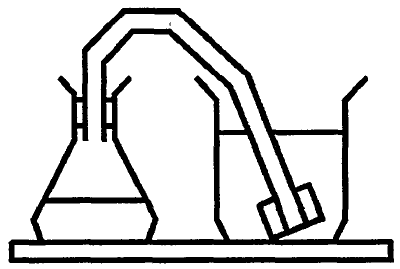
\includegraphics[width=6cm]{gfx/beauty97-1.png}
	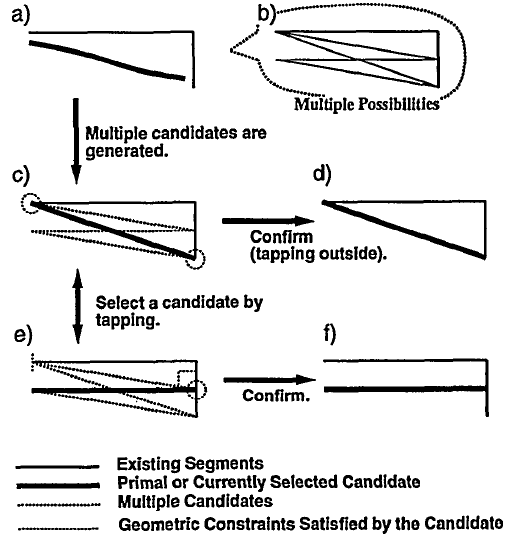
\includegraphics[width=6.5cm]{gfx/beauty97-2.png}
	\caption{Pegasus: A diagram drawn on Pegasus without using any editing commands such as rotation, copy or gridding (left); interaction with multiple candidates (right).}
	\label{FIG-PEGASUS}
\end{figure}

\subsubsection{Discussion}

TODO
%(PEGASUS): The technique appears to be of great use in my project - in architecture most walls subsume these constraints.
%Additionally my users will model in 3D, which increases the interest in applying beautification algorithms
%such as this one.

\subsection{Navigation}

\subsubsection{Smart and Physically Based Navigation}
In order to ensure users not ''getting lost'' in the virtual space, Buchholz, Bohnet and D�llner \cite{SMARTCAM05} propose
a camera that is is both smart and physically-based. Smart in the sense that it is aware of confusing,
disorienting viewing situations and provides means to circumvent them. Physically based because it is
supported by a physically based model of the 3D motion to ensure steady, continuous user movements.

In order to solve the disorientation problem the camera has to identify situations when to intervene. For that
matter a metric, called orientation value, was created. Each view is classified by counting its pixels, granting
different scores: highest values for landmarks; high values for terrain; low values for the sky.
Therefore a threshold can be established and views below it are classified ''disoriented''.

When such an event takes place, smart navigation techniques restrict camera control. The constraints posed
to user control must be as comprehensible as possible. Camera movement should also be time-coherent and physically sound.

The maintenance strategy solves critical situations such as (see Figure \ref{FIG-SMARTCAM1}, left):

\begin{enumerate}[a)]
	\item The user rotates the flight direction and causes the camera to look too far beyond the terrain border.
		The rotation is accepted but outweighed by a slight rear movement away from the border.
	\item The user is flying forward beyond the terrain border.
		The maintenance strategy temporarily tilts down the view direction until a maximum angle is reached.
	\item If no more tilting is possible, the strategy rotates the flight direction parallel to the terrain
		to fly along the terrain border.
\end{enumerate}

\begin{figure}[htb]
	\centering
	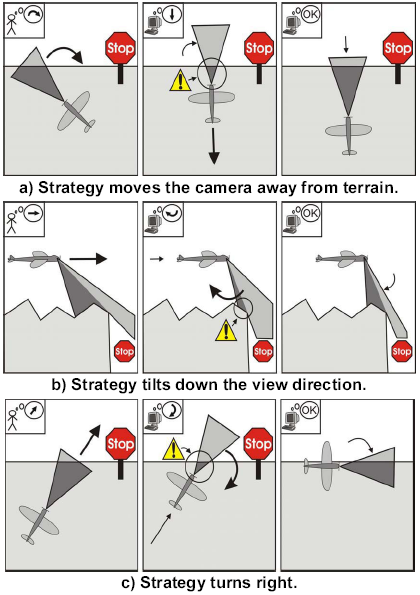
\includegraphics[width=5cm]{gfx/smartcam05-1.png}
	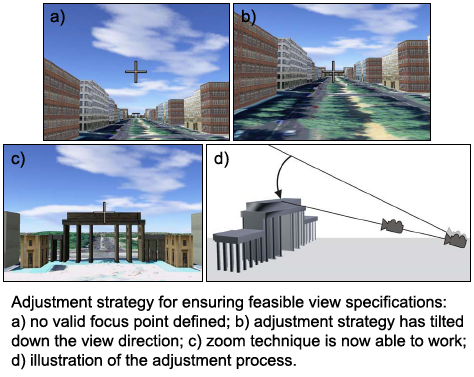
\includegraphics[height=3cm]{gfx/smartcam05-2.png}
	\caption{SPB Cam: Maintenance strategy for keeping high orientation values (left); Adjustment strategy for ensuring of feasible view specifications (right).}
	\label{FIG-SMARTCAM1}
\end{figure}

TODO end article!


%\subsubsection{}

%\cite{SKAN02}
%\cite{DESFUT04}

